\documentclass{article}
%%%%%%%%%%%%%%%%%%%%%%%%%%%%%%%%%%%%%%%%%%%%%%%%%%%%%%%%%%%%%%%%%%%%%%%%%%%%%%%%%%%%%%%%%%%%%%%%%%%%%%%%%%%%%%%%%%%%%%%%%%%%%%%%%%%%%%%%%%%%%%%%%%%%%%%%%%%%%%%%%%%%%%%%%%%%%%%%%%%%%%%%%%%%%%%%%%%%%%%%%%%%%%%%%%%%%%%%%%%%%%%%%%%%%%%%%%%%%%%%%%%%%%%%%%%%
\usepackage{amsmath,amssymb}
% more math
\usepackage{amsfonts}
\usepackage{amssymb}
\usepackage{amstext}
\usepackage{amsbsy}

\usepackage{float}
\usepackage{graphicx}
\usepackage{color}
\newcommand{\mt}[1]{\marginpar{\small #1}}
%%%%%%%%%%%%%%%%%%%%%%%%%%%%%%%%%%%%%%%%%%%%%%%%%%%%%%%%%%%%%%%%%%%%
% new commands
\newcommand{\nc}{\newcommand}
% operators
\renewcommand{\div}{\vec{\nabla}\! \cdot \!}
\newcommand{\grad}{\vec{\nabla}}
% latex shortcuts
\newcommand{\bea}{\begin{eqnarray}}
\newcommand{\eea}{\end{eqnarray}}
\newcommand{\be}{\begin{equation}}
\newcommand{\ee}{\end{equation}}
\newcommand{\bal}{\begin{align}}
\newcommand{\eali}{\end{align}}
\newcommand{\bi}{\begin{itemize}}
\newcommand{\ei}{\end{itemize}}
\newcommand{\ben}{\begin{enumerate}}
\newcommand{\een}{\end{enumerate}}
% DGFEM commands
\newcommand{\jmp}[1]{[\![#1]\!]}                     % jump
\newcommand{\mvl}[1]{\{\!\!\{#1\}\!\!\}}             % mean value
\newcommand{\keff}{\ensuremath{k_{\textit{eff}}}\xspace}
% shortcut for domain notation
\newcommand{\D}{\mathcal{D}}
% vector shortcuts
\newcommand{\vo}{\vec{\Omega}}
\newcommand{\vr}{\vec{r}}
\newcommand{\vn}{\vec{n}}
\newcommand{\vnk}{\vec{\mathbf{n}}}
\newcommand{\vj}{\vec{J}}
% extra space
\newcommand{\qq}{\quad\quad}
% common reference commands
\newcommand{\eqt}[1]{Eq.~(\ref{#1})}                     % equation
\newcommand{\fig}[1]{Fig.~\ref{#1}}                      % figure
\newcommand{\tbl}[1]{Table~\ref{#1}}                     % table

\newcommand{\ud}{\,\mathrm{d}}

\newcommand{\tcr}[1]{\textcolor{red}{#1}}
%%%%%%%%%%%%%%%%%%%%%%%%%%%%%%%%%%%%%%%%%%%%%%%%%%%%%%%%%%%%%%%%%%%%

\begin{document}

\begin{center}
{ \Large Answers to Reviewer \#1}
\end{center}

\bigskip

\noindent Ms. Ref. No. JCOMP-D-13-00928\\
Discontinuous Finite Element Solution of the Radiation Diffusion Equation on Arbitrary Polygonal Meshes and Locally Adapted Quadrilateral Grids\\
{\it Journal of Computational Physics},\\

\bigskip
\bigskip

{
\color{blue}
This paper is a very high quality paper for the Journal of Computational Physics and should be
accepted for publication without reservation. One of the main strengths of this paper is its very thorough
review of spatial discretization technology for radiation diffusion. It is well written, and includes a
comprehensive set of test problems applied to the new discretization proposed.
}

Thank you for your thorough review and appreciation of our work. 
\bigskip


{
\color{blue}
I have some suggestions for improvement, but as a reviewer, I do not require these additions to the paper
for publication.
}


Thank you. Even though you do not require these additions for publication, I wish to publish the best 
possible papers and I will include as many suggestions for improvement as possible in the revised version of 
this manuscript.
\bigskip



{
\color{blue}
On the list or prior works, a reference or references should be included for each item in the list. For the
first two items, no references are included.
}

In this short enumeration of prior works, our intent was not to add new references but to recall
the various techniques we have just reviewed in the above paragraphs. However, we have forgotten to 
discuss FV techniques for polygonal meshes. This is now corrected and a sentence has been added in the 
above literature review. Mimetic FD were already described and reviewed above so we do not think we are missing 
references for this type of discretization techniques. 
\bigskip

{
\color{blue}
The derivation of the discretization is complicated enough to warrant an appendix which goes through
the details of the mathematics (e.g. how to get to Eq. 3 and Eq. 8), like one would find in a thesis or
dissertation. I am a proponent of including these detailed types of explanations in papers because I think
they enhance the read-ability of the paper; however, some disagree with this philosophy.
}


The review article ``Unified Analysis of Discontinuous Galerkin Methods for Elliptic Problems'' (Douglas et. al.),
the habilitation thesis ``Discontinuous Galerkin Methods for Viscous Incompressible Flow'' by Kanschat and a SIAM book on DG 
methods that we have added in the revised manuscript ``Discontinuous Galerkin Methods for Solving Elliptic and Parabolic Equations: 
Theory and Implementation'' by Rivi\`ere are several resources that provide an excellent description of the SIP method for 
elliptic problems (along with other DG variants). 
\bigskip

{
\color{blue}
The author could state more clearly how this work is distinct from previous work. The author mentions
that others have applied a Discontinuous method to diffusion operators. How is the proposed method
different? In section 3, the author writes: "Many variants of such discontinuous discretization methods
exist for diffusion problems…" It may be a good idea to say, the discretization in this paper is different
because…
}

The DG technique for the radiation diffusion equation is the standard Symmetric Interior Penalty (SIP) technique. 
We have chosen it because it yields a symmetric linear system that can be efficiently solved using
a preconditioned conjugate gradient technique. The novelties are: the use SIP on polygonal meshes, hence the use of the PWLD basis functions,
and adaptive mesh refinement carried out with with PWLD resulting in polygonal meshes.

\bigskip

{
\color{blue}
I am curious as to why the statement was made that "we have opted to use two loops: one over the
elements…" Did this have an impact of computational performance? It seems like the reason why was never
addressed.
}

The DG bilinear form, Eq.(8), may look a bit complex. It contains volume integrals (or surface integral in 2D geometry)
and face integrals (edge integrals in 2D). The volume integrals are split on each element (thus we loop over the elements). 
Each volume integral for a given element only contribute entries in the global matrix for the unknowns present 
in that element (a feature of DG methods). The face integrals are split over the faces (thus we loop over the set of interior faces). 
Each face integral contributes entries in the global matrix for the  unknowns present in the two elements separated by that face. 
Thus, the manner in which cell/face information is accessed and used is different and we felt that implementing these volume/surface contributions
to the global matrix would make the code clearer. One can of course one a single loop over elements and, for a given element, deal 
with the face integral pertaining to that element at that moment.

We haven't assessed the impact on computational performance for either of these two implementations (we have coded only one implementation).

\bigskip

{
\color{blue}
For the discussion at the top of page 9 about C and h$_\perp$ a picture may be helpful, especially when
describing the inradius and circumradius for polygons.\\
}
The constant $C$ needs to be of order 1 for the SIP method; this is described in the SIP references of Kanschat and the 
book of Rivi\`ere. We have added a note (and a reference) pertaining to another interior penalty method where $C$ can be 0; however,
in this case the resulting linear system is nonsymmetric and cannot be tackled using a preconditioned conjugate gradient technique.
We believe that the interested readers will find adequate information in the references we cite in the introduction and in that 
particular section of the manuscript.\\


The definitions for the inradius and the circumradius for regular polygons are standard.
The figures below summarize the values of $h_\perp$ for a regular polygons using a pentagon and a hexagon as examples of polygons 
with odd and even number of sides. In the manuscript, we added that
the formulae used to compute the inradius and the circumradius based on a regular polygon's area and perimeter
are used for any polygon. What really matters is the value of the resulting penalty coefficient.  

\begin{figure}[H]
\centering
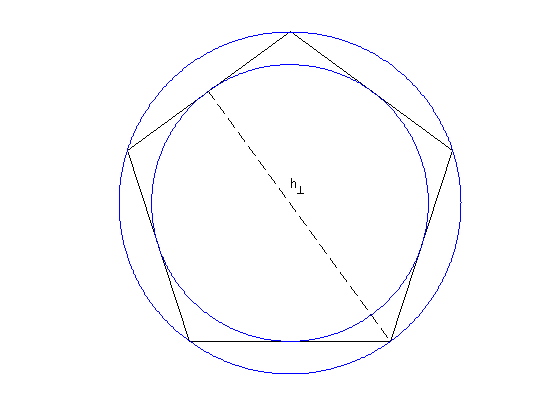
\includegraphics[scale=0.75]{hperp_odd.png}
\end{figure}
\begin{figure}[H]
\centering
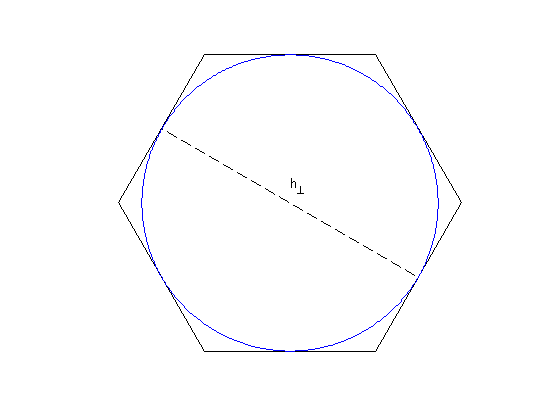
\includegraphics[scale=0.75]{hperp_even.png}
\end{figure}


\bigskip


{
\color{blue}
I am curious if the author has tried standard linear basis functions (u(x,y) = a + bx + cy) on
quadrilaterals to see if this works for the DFEM type diffusion discretization.
}

One can, of course, use linear basis functions on quadrilaterals. However, the ultimate goal is to employ
the diffusion solver as a synthetic preconditioner for radiation transport solves. In the thick diffusion limit,
employing linear basis functions on quadrilaterals leads to a locking of the transport solution to the 
wrong answer. In reactor problems, where the thick diffusion limit is not a relevant regime, researchers
may prefer to use linear basis functions (a+bx+cy+dz) on hexadredal cells to reduce the number of unknowns
without drastically reducing accuracy.

\bigskip

{
\color{blue}
What code was this method implemented in? Was it just a test code? Was it MATLAB? Were there any
parallel runs? What linear solver package was used, if any?
}

The test bed code is MATLAB. We use both the built-in optimized LU package but also a conjugate gradient solve
preconditioned with an algebraic multigrid method. The PWLD SIP technique for diffusion is now being 
implemented in a massively C++ radiation transport to be used either as a standalone solver or a 
synthetic preconditioner for transport solves. 



\bigskip


{
\color{blue}
I think a potential weakness of the paper is that the author does not compare the new method to any of
the existing methods. If this is not hard to do, these results would be very interesting to include in the
paper. Additionally, these results could be included in a future paper or conference proceedings.
}

We haven't implemented mimetic finite differences or Palmer's method so we cannot compare with them. We are
currently implementing the SIP discretization of the diffusion equation with PWLD basis functions 
in our parallel transport solver, PDT.  In PDT, we already have a PWLC (C for continuous)
finite element discretization of the diffusion equation for polygonal grids. We expect to communicate in the near
future DSA results comparing PWLD-SIP versus PWLC (which requires a discontinuous update as a post-processing step to
be an effective preconditioner).
 \bigskip


{
\color{blue}
For the linear test problem results, what are the iteration counts for the linear solve as the mesh is
distorted? Was the iteration count a lot different for the different mesh types? For quads vs. polygons?
}


Most of the results are obtained through MATLAB's LU direct solve but we have also implemented a PCG preconditioned with AMG 
(aggregation multigrid method or AGMG). For a CG tolerance of $10^{-11}$, the number of PCG iterations was: 20 (quad mesh),
74 (Z-mesh quad), and 73 (Z-mesh poly). So, the polygon type (quad versus arbitrary polygons) has little impact on
the iterative efficiency on heavily distorted meshes.
\bigskip


{
\color{blue}
A reference for computing bounded Voronoi diagrams is a good idea.
}


It is well known that the boundaries of a Voronoi diagram may have line segments of infinite length. By bounded Voronoi diagram, 
we simply mean that we bound these line segments to intersect the  bounded box of the original quadrilateral mesh. 
We are not aware of a reference for this. The idea in itself is simple. We illustrate it below: in red, we have a triangular mesh 
in the rectangle $-6 \le x\,,y \le 6$. The blue lines represent the standard Voronoi diagram. We simply bound Voronoi diagram by 
the original rectangular domain.

\begin{figure}[H]
\centering
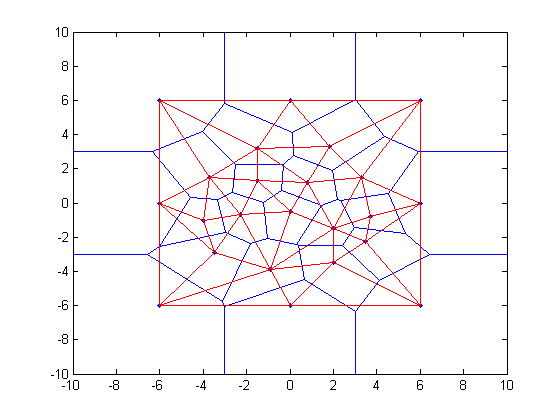
\includegraphics[scale=0.75]{bounded_voronoi_example.png}
\end{figure}
\begin{figure}[H]
\centering
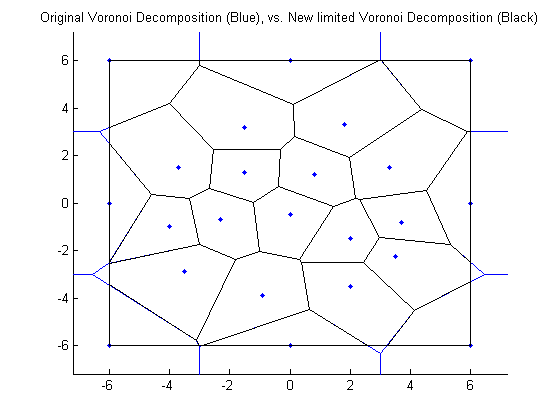
\includegraphics[scale=0.75]{bounded_voronoi_example2.png}
\end{figure}
% for a set of points (here, vertices of quadrangular meshes)

\bigskip




{
\color{blue}
For the convergence plots, I think the terminology is a bit inconsistent. In the text the author writes
in terms of dof. In the plots, he uses number of unknowns. This could be a bit more consistent, but is a
minor detail.
}

Just before Eq.(23), we mentioned degrees of freedom and unknowns concurrently in the same sentence. But it is true
that we use predominantly the term ``unknowns''. We have modified the manuscript accordingly.

\bigskip


{
\color{blue}
In general, an understanding of how resistant this method is to negative solutions would be another
interesting thing to study, especially in a time dependent case, with a delta-function like source. I would
anticipate that this method would perform a lot better than the CFEMs.
}

We will keep this in mind but believe this topic is outside of the scope of the current manuscript. Thank you
for the suggestion.
\bigskip



{
\color{blue}
Does the author anticipate a straight-forward application to RZ geometry and 3D geometry? Will the
method recover spherical symmetry in RZ geometry. Brunner, et. Al. have observed an issue with this for RZ
geometry. See T.A. Brunner…, "Preserving Spherical Symmetry in Axisymmetric Coordinates for Diffusion,"
in Proc. International Conference on Mathematics and Computational Methods Applied to Nuclear Science and
Engineering, May 5-9, 2013, Sun Valley, ID (2013), CD-ROM
}

We haven't looked into this issue yet but will look forward to investigating it, including porting SIP PWLD in RZ geometries
for radiation diffusion problems.
\bigskip


\end{document}

